\documentclass[a4paper]{article}
\usepackage{amsmath}
\usepackage{graphicx}
\usepackage{geometry}
\usepackage{floatrow}
\usepackage{layout}
\usepackage{amssymb} 
\usepackage{multirow}
\usepackage{caption}
\geometry{margin=1in}
\usepackage{authblk}
\usepackage{indentfirst}
\usepackage[hidelinks]{hyperref}
\usepackage{enumitem}
\usepackage{float}
\usepackage{hyperref}
\usepackage{amssymb}
\usepackage{xcolor}
\usepackage{titlesec}

% Define link color
\hypersetup{
    colorlinks=true,
    linkcolor=teal,  % Color for internal links
    filecolor=teal,  % Color for file links
    urlcolor=teal,   % Color for URLs
    citecolor=black  % Color for citation links
}

% Define custom dark teal color
\definecolor{darkteal}{RGB}{0, 102, 102} % Adjust the RGB values as needed

% Define section color
\titleformat{\section}
  {\color{darkteal}\normalfont\Large\bfseries} % Formatting for section titles
  {\thesection}{1em}{}

\providecommand{\keywords}[1]
{
  \small	
  \textbf{\; \textit{Keywords---}} #1
}

\begin{document}

\title{\textbf{\huge{Problem Set 1}}}

\author{\textbf\large{Teera Tesharojanasup}}

\affil{\textbf{Northeastern University, Boston}}

\date{\text{July 10th, 2024}}

\maketitle
\begin{sloppypar}

\section*{Overview}

Problem set 1 for CS 4100 Summer II. Taught by assistant teaching professor, \href{https://rajagopalvenkat.com/}{Rajagopal Venkat}. \cite{MISC:1}

\section{Categorizing AI Environments}

\begin{enumerate}[start=1,label=Q\arabic*,left=0pt]
    \item \textbf{Under what (implementation-related) assumptions is maze-solving a fully observable environment? What are the agent’s percepts? \hfill \textcolor{teal}{(2)}}
    
    \par 
    
    \item \textbf{Under what (implementation-related) assumptions is maze-solving a partially observable environment? What are the agent’s percepts? \hfill \textcolor{teal}{(2)}}
    
    \par
    
    \item \textbf{Is a known environment always fully observable? Explain with an example. \hfill \textcolor{teal}{(2)}}
    
    \par
    
    \item \textbf{Is a partially observable environment always an unknown environment? Explain with an example. \hfill \textcolor{teal}{(2)}}
    
    \par 

    \item \textbf{What is the difference between an unknown environment and a non-deterministic environment? Explain with an example. \hfill \textcolor{teal}{(2)}}
    
    \par
    
\end{enumerate}

\section{Search}

In this problem set, we will be using Rook Jumping Mazes (RJMs) - a game based on
Rook moves in Chess - to understand various search techniques. In a RJM, you are
given a square $n \times n$ grid, with each cell containing a number between $1$ to $n - 1$. From
any cell, the player may move either horizontally or vertically but must take exactly the
number of steps as shown on the player’s current cell. Regardless of the length of the
jump (i.e. number of cells passed), this action is considered a single jump (i.e., having a
cost of 1) for purposes of our search. The objective is to get from an assigned start state
to a pre-specified goal state. Consider this example:

\begin{figure}[H]
    \centering  
    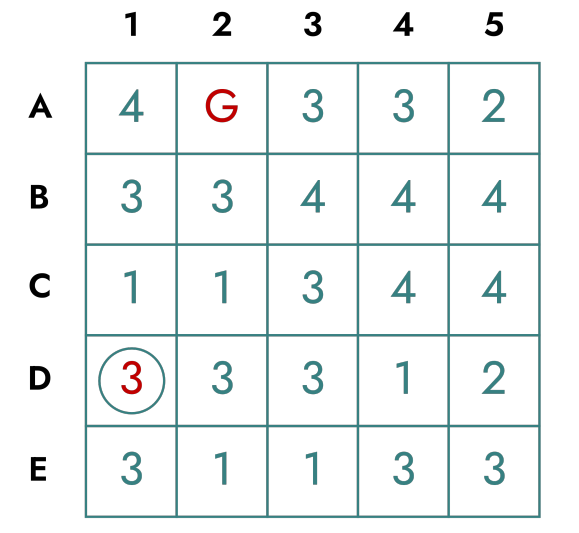
\includegraphics[height=0.2\textheight]{Search_RJM.png}
    \label{fig:Search_RJM}
\end{figure}

\noindent The cell D1 is the start state and the cell A2 is the goal state. The shortest solution to this
RJM is: [D1, A1, A5, C5, C1, C2, D2, A2]. Such a game lends itself well to the various
search algorithms we covered in class.

\begin{enumerate}[start=6,label=Q\arabic*,left=0pt]
    \item \textbf{Can both Breadth-First Search (BFS) and Depth-First Search (DFS) be used to solve RJMs? Will both yield the shortest path? \hfill \textcolor{teal}{(2)}}
    
    \par

    \item \textbf{Assuming that each jump has a cost of 1, irrespective of the number of cells the rook
    passes while making that jump, we can use A* search to find the shortest path. Recall
    from class that A* search requires a consistent heuristic to guarantee an optimal solution.
    Show that for this problem, the Manhattan distance from any cell to the goal cell divided
    by (n - 1) is a consistent heuristic, where n is the number of cells in a row/column. In other words, show that}

    \[ H(node, goal, n) = \frac{|node_x - goal_x| + |node_y - goal_y|}{n - 1} \]

    \textbf{is a consistent heuristic. Remember that a proof may not rely on a single example, but instead must hold true in general. \hfill \textcolor{teal}{(5)}}
    
    \par
    
    \item \textbf{Consider the following RJM:}
    \begin{figure}[H]
        \centering  
        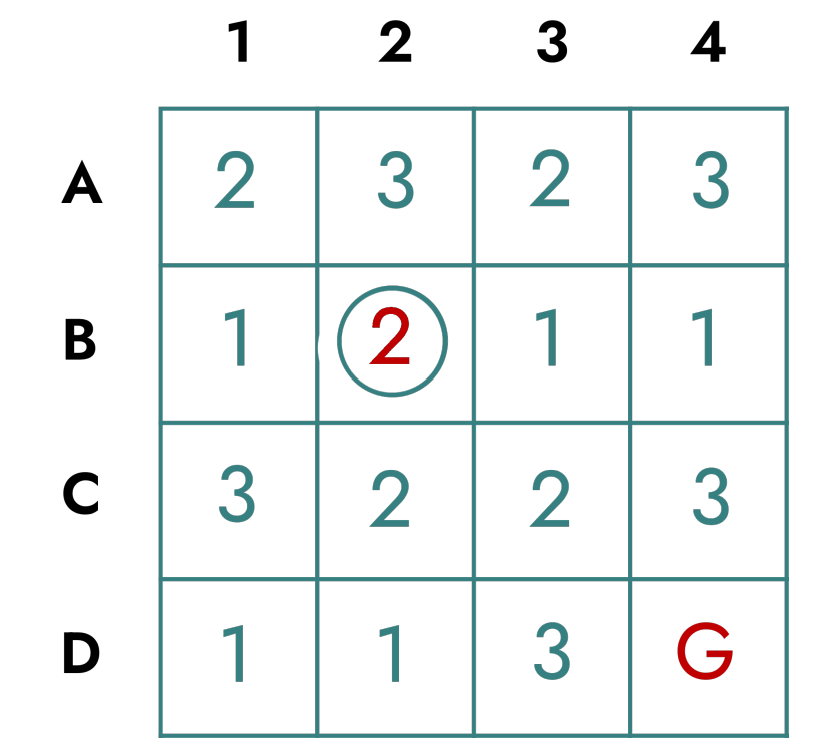
\includegraphics[height=0.2\textheight]{Q8_RJM.png}
        \label{fig:Q8_RJM}
    \end{figure}

    \textbf{On this maze, using the heuristic from Q7, complete the A* search process shown be- low, starting with Step 2. Terminate your search when the Goal node (cell D4) is popped from the priority queue. Double check your calculations! \hfill \textcolor{teal}{(8)}}
    
    \par

\end{enumerate}

\section{Local Search}

Your professor is a coffee snob, and since he knows a thing or two about AI, he tries to
build an espresso machine that will learn a user’s preferences over time to pull the perfect
shot. He lets the machine control the following values:

\begin{itemize}
    \item Weight of coffee beans (15-21 grams)
    \item Grind size (250 - 400 microns)
    \item Water Pressure (7 - 11 bars)
    \item Brew time (27 - 33 seconds)
\end{itemize}

\begin{enumerate}[start=9,label=Q\arabic*,left=0pt]
    \item \textbf{Based on our discussions in class, is this problem well-suited to local search algorithms? Explain your reasoning. \hfill \textcolor{teal}{(2)}}
    
    \par 
    
    \item \textbf{How you would implement such a program? What would be a reasonable objective function? (This question is somewhat open-ended, so don’t worry too much about the ‘right’ answer. I am really looking for whether your thought process reflects a solid understanding of how local search works.) \hfill \textcolor{teal}{(2)}}
    
    \par

    \item \textbf{Which of the optimizations and local search variants discussed in class (random restarts, varying step size, simulated annealing and genetic algorithms) are applicable to this problem, and why? \hfill \textcolor{teal}{(2)}}
    
    \par 

\end{enumerate}

\section{Adversarial Search}

\begin{enumerate}[start=12,label=Q\arabic*,left=0pt]
    \item \textbf{Construct a game tree example with a depth of 4 and a branching factor of 2, that illustrates the best-case for alpha-beta pruning, except for the trivial solution. Hand drawn figures accepted for this question, but please ensure clarity. 
    (Here's some inspiration: \href{https://science.slc.edu/~jmarshall/courses/2005/fall/cs151/lectures/minimax/BestCase.html}{CS151, 2005. Jim Marshall, SLC}) \hfill \textcolor{teal}{(2)}}

    \item \textbf{Why is it desirable to combine iterative deepening with alpha-beta pruning from a practical standpoint? \hfill \textcolor{teal}{(2)}}
    
    \par 

\end{enumerate}

\section{Academic Integrity}

\begin{enumerate}[start=14,label=Q\arabic*,left=0pt]
    \item \textbf{Review, and copy/paste the academic integrity acknowledgement in your final submission as the answer to Q14.}
    \par I have read and understood the academic integrity policy as outlined in the course syllabus for CS4100. 
    By pasting this acknowledgement in my submission, I declare that all work presented here is my own, 
    and any conceptual discussions I may have had with classmates have been fully disclosed. I declare that generative AI 
    was not used to answer any questions in this assignment. Any use of generative AI to improve writing clarity 
    alone is accompanied by an appendix with my original, unedited answers.
\end{enumerate}
\end{sloppypar}

\bibliography{references}
\bibliographystyle{ieeetr}

\end{document}